\part{Desenvolvimento}
\chapter{Arquitetura da Plataforma}
\section{Estrutura do Projeto}

\subsection{Raiz do Projeto}
\begin{itemize}
\item \textbf{README.md:} Documentação do projeto em formato markdown.
\item \textbf{pnpm-lock.yaml:} Arquivo de lock para gerenciar dependências com o gerenciador de pacotes pnpm.
\item \textbf{middleware.ts:} Middleware utilizado para determinar se as paginas são de acesso publico ou se devem passar pela autenticação.
\item \textbf{.env.local e .env:} Variáveis de ambiente
\item \textbf{.gitignore:} Lista de arquivos e pastas a serem ignorados pelo Git durante o versionamento.
\item \textbf{.git:} Pasta do repositório Git, onde são armazenados os metadados do controle de versão.
\item \textbf{package.json:} Arquivo de configuração do Node.js que descreve o projeto e suas dependências.
\item \textbf{components.json:} Arquivo de configuração de componentes do ShadCN UI.
\item \textbf{tsconfig.json:} Configuração do TypeScript para o projeto.
\item \textbf{postcss.config.js:} Configuração do PostCSS para processamento de estilos.
\item \textbf{.eslintrc.json:} Configurações do ESLint para linting e padronização de código.
\item \textbf{next-env.d.ts:} Declarações de tipos do Next.js para TypeScript.
\item \textbf{tailwind.config.ts:} Configurações específicas do Tailwind CSS.
\item \textbf{next.config.js:} Arquivo de configuração do Next.js para customizações no ambiente.
\item \textbf{public:} Pasta de arquivos publicos como imagens utilizadas no projeto.
\item \textbf{app:} Pasta que contém componentes, páginas e recursos relacionados à estrutura geral do aplicativo. \ref{app}
\item \textbf{prisma:} Pasta que contem as configurações do ORM Prisma. \ref{prisma}
\item \textbf{server:} Pasta que contem a estrutura do servidor com TRPC, autenticação e banco de dados. \ref{server}
\end{itemize}

\subsection{App}
\label{app}
\begin{itemize}
\item \textbf{sign-up:} Página de cadastro.
\item \textbf{sign-in:} Página de login.
\item \textbf{terms-of-use:} Página de termos de uso.
\item \textbf{privacy-policy:} Página de política de privacidade.
\item \textbf{terapeuta:} Página do terapeuta e todos os seus componentes.
\item \textbf{participante:} Pagina do participante e todos os seus componentes.

\item \textbf{posthog:} Pasta de configuração e criação de um provider para o PostHog.
\item \textbf{trpc:} Configuração de um cliente TRPC que possa ser utilizado tanto em componentes com renderização no servidor ou no cliente.
\item \textbf{lib:} Funções e utilitários compartilhados.
\item \textbf{components:} Componentes reutilizáveis.


\item \textbf{api:} Pasta para lidar com rotas da API.
\begin{itemize}
\item \textbf{trpc:} Rotas TRPC específicas.
\item \textbf{clerk:} Possível roteamento para recursos relacionados ao Clerk.
\end{itemize}

\item \textbf{layout.tsx:} Layout comum a todas as paginas, inclui o provider do PostHog, TRPC e de Autenticação.
\item \textbf{globals.css:} Arquivo de estilos globais.
\item \textbf{favicon.ico:} Ícone exibido na barra de título do navegador.
\end{itemize}


\subsection{Prisma}
\label{prisma}
\begin{itemize}
\item \textbf{schema.prisma:} Arquivo de definição de modelo para o Prisma ORM.
\end{itemize}

\subsection{Server}
\label{server}
\begin{itemize}
\item \textbf{routers:} Rotas relacionadas a diferentes recursos, como vídeos, grupos e usuários.
\item \textbf{trpc.ts:} Configuração de chamadas publicas e protegidas na comunicação TRPC
\item \textbf{index.ts:} Ponto de entrada do servidor.
\item \textbf{db.ts:} Arquivo de configuração ou conexão com o banco de dados.
\end{itemize}


\section{Fluxo de autenticação OAuth 2.0}
% \subsection{A implementação da autenticação \textit{OAuth 2.0}}
O \textit{OAuth} 2.0 é o protocolo central que representa um pilar sólido de segurança e o gerenciamento eficaz dos acessos às sessões de TCI na plataforma. Este protocolo de autorização é fundamental para o processo, permitindo que a plataforma obtenha acesso limitado a contas de usuários em serviços \textit{Hypertext Transfer Protocol} (HTTP) sem a necessidade de enviar diretamente usuário e senha. Em essência, o usuário delega a um determinado aplicativo acesso aos seus dados em um serviço ou API específicos.\cite{OAUTH}Ao adotar o \textit{OAuth} 2.0 do Google neste projeto, não apenas garante um método confiável para autenticar usuários, mas também preserva a integridade dos dados, permitindo que somente usuários autorizados tenham acesso à plataforma. Essa escolha tecnológica não só oferece solidez ao processo de autenticação, mas também acrescenta uma camada adicional de segurança ao ambiente da plataforma.

No contexto do fluxo de autenticação, desde o redirecionamento do navegador até a obtenção e validação do \textit{token} de acesso, há uma atenção especial às considerações de usabilidade. Durante o processo de login, a plataforma direciona o navegador para um \textit{Uniform Resource Locator}URL do Google, incorporando parâmetros que indicam o tipo de acesso desejado. Nesse momento, o usuário realiza o login com a Conta do Google, seleciona a sessão e, crucialmente, concede as permissões necessárias. Após o login, o usuário é solicitado a confirmar se deseja conceder as permissões requisitadas pela plataforma. A inclusão desses elementos visa não apenas garantir a segurança, mas também oferecer uma experiência de usuário intuitiva e transparente. Abaixo uma imagem exemplificando o fluxo de autenticação realizado pelo \textit{OAuth} 2.0 do Google\cite{OAUTHACESS}:

\begin{figure}[!ht] % ambiente usado para inserção de imagens
    \centering
    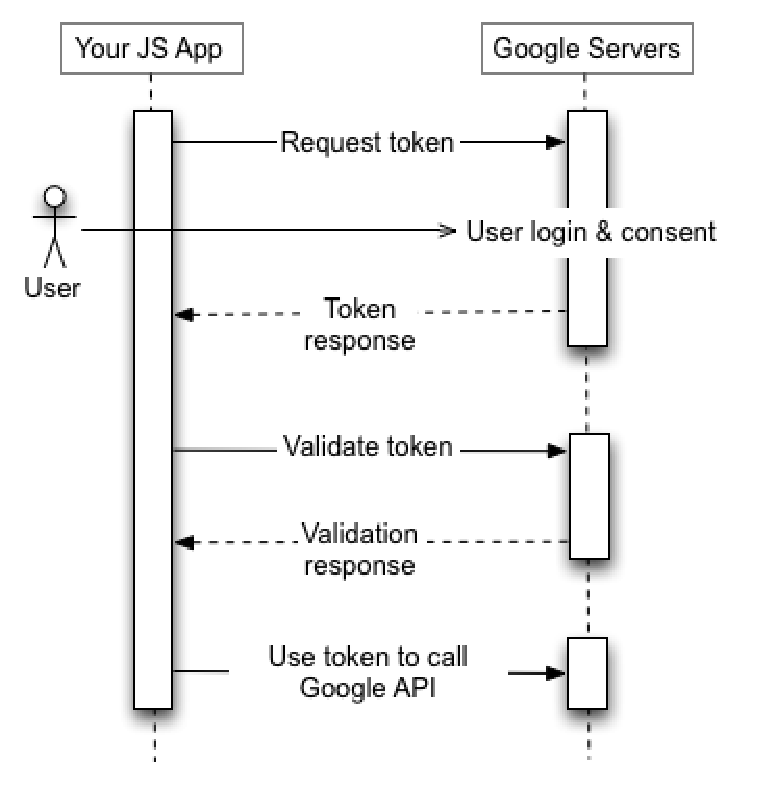
\includegraphics[scale=0.5]{latex/figuras/oauth.pdf}
    \caption[Fluxo de autenticação OAuth 2.0 do Google]
    {Fluxo de autenticação realizado pelo OAuth 2.0 do Google}
\end{figure}

\pagebreak Além disso, a abordagem dos escopos provenientes do protocolo OAuth 2.0 do Google destaca-se como um componente crucial da estratégia de permissões. A inclusão desses escopos na resposta do token desempenha um papel vital para acessar recursos específicos do projeto, alinhando as escolhas tecnológicas com a usabilidade da plataforma. Dessa forma, os usuários fornecem apenas o essencial para o acesso aos recursos e funcionalidades pertencentes ao projeto, contribuindo para uma experiência mais personalizada e segura. A seguir, apresenta-se a relação de escopos provenientes do protocolo OAuth 2.0 do Google, os quais foram empregados no desenvolvimento da plataforma \cite{OAUTHSCOPES}:

\begin{itemize}
\item \textit{\textbf{openId}} → Associação do usuário às suas informações pessoais presentes no Google

\item \textit{\textbf{userinfo.email}} → Visualização do endereço de e-mail principal associado à Conta do Google

\item \textit{\textbf{userinfo.profile}} → Acesso e visualização de informações pessoais, incluindo aquelas disponibilizadas publicamente;
\item \textit{\textbf{calendar}} → Permissão para gerenciar todas as agendas às quais o usuário tem acesso por meio do Google Calendar.
\end{itemize}

Os \textit{tokens} de acesso são válidos somente para o conjunto de operações e recursos descritos no escopo. Por exemplo, está sendo usado na plataforma um \textit{token} de acesso emitido para a API Google Calendar, ele não concederá acesso à uma API \textit{Google Contacts}. O aplicativo precisa armazenar o \textit{token} de atualização para uso futuro e usar o \textit{token} de acesso para acessar uma API do Google. Quando o \textit{token} de acesso expira, o aplicativo usa o \textit{token} de atualização para conseguir um novo.

Para complementar, a política de expiração definida para os \textit{tokens} foi um tempo de 24 horas para o \textit{token} de atualização e um tempo mais curto, 30 minutos, para o \textit{token} de acesso, evidenciando uma consideração equilibrada de usabilidade e segurança. Essa abordagem visa não apenas a proteção contra acessos não autorizados, mas também a otimização da experiência do usuário, evitando logins frequentes.

Assim, as escolhas tecnológicas incorporadas na implementação do \textit{OAuth} 2.0 refletem uma busca constante por segurança robusta, ao mesmo tempo em que priorizam uma experiência do usuário coesa e eficiente na plataforma.

\section{Fluxo de Desenvolvimento do Projeto}

    No processo de construção da plataforma para facilitar o acesso aos grupos de Terapia Comunitária Integrativa Online, \textit{stories} e \textit{epics} delimitam a narrativa do projeto. \textit{Stories} são tarefas detalhadas, enquanto \textit{epics} agrupam objetivos amplos. Esse fluxo inicia-se com a definição de \textit{epics}, desdobrando-se em \textit{stories}. Abaixo, é possível visualizar as etapas de desenvolvimento do projeto:\\
\begin{figure}[!ht]
    \centering
    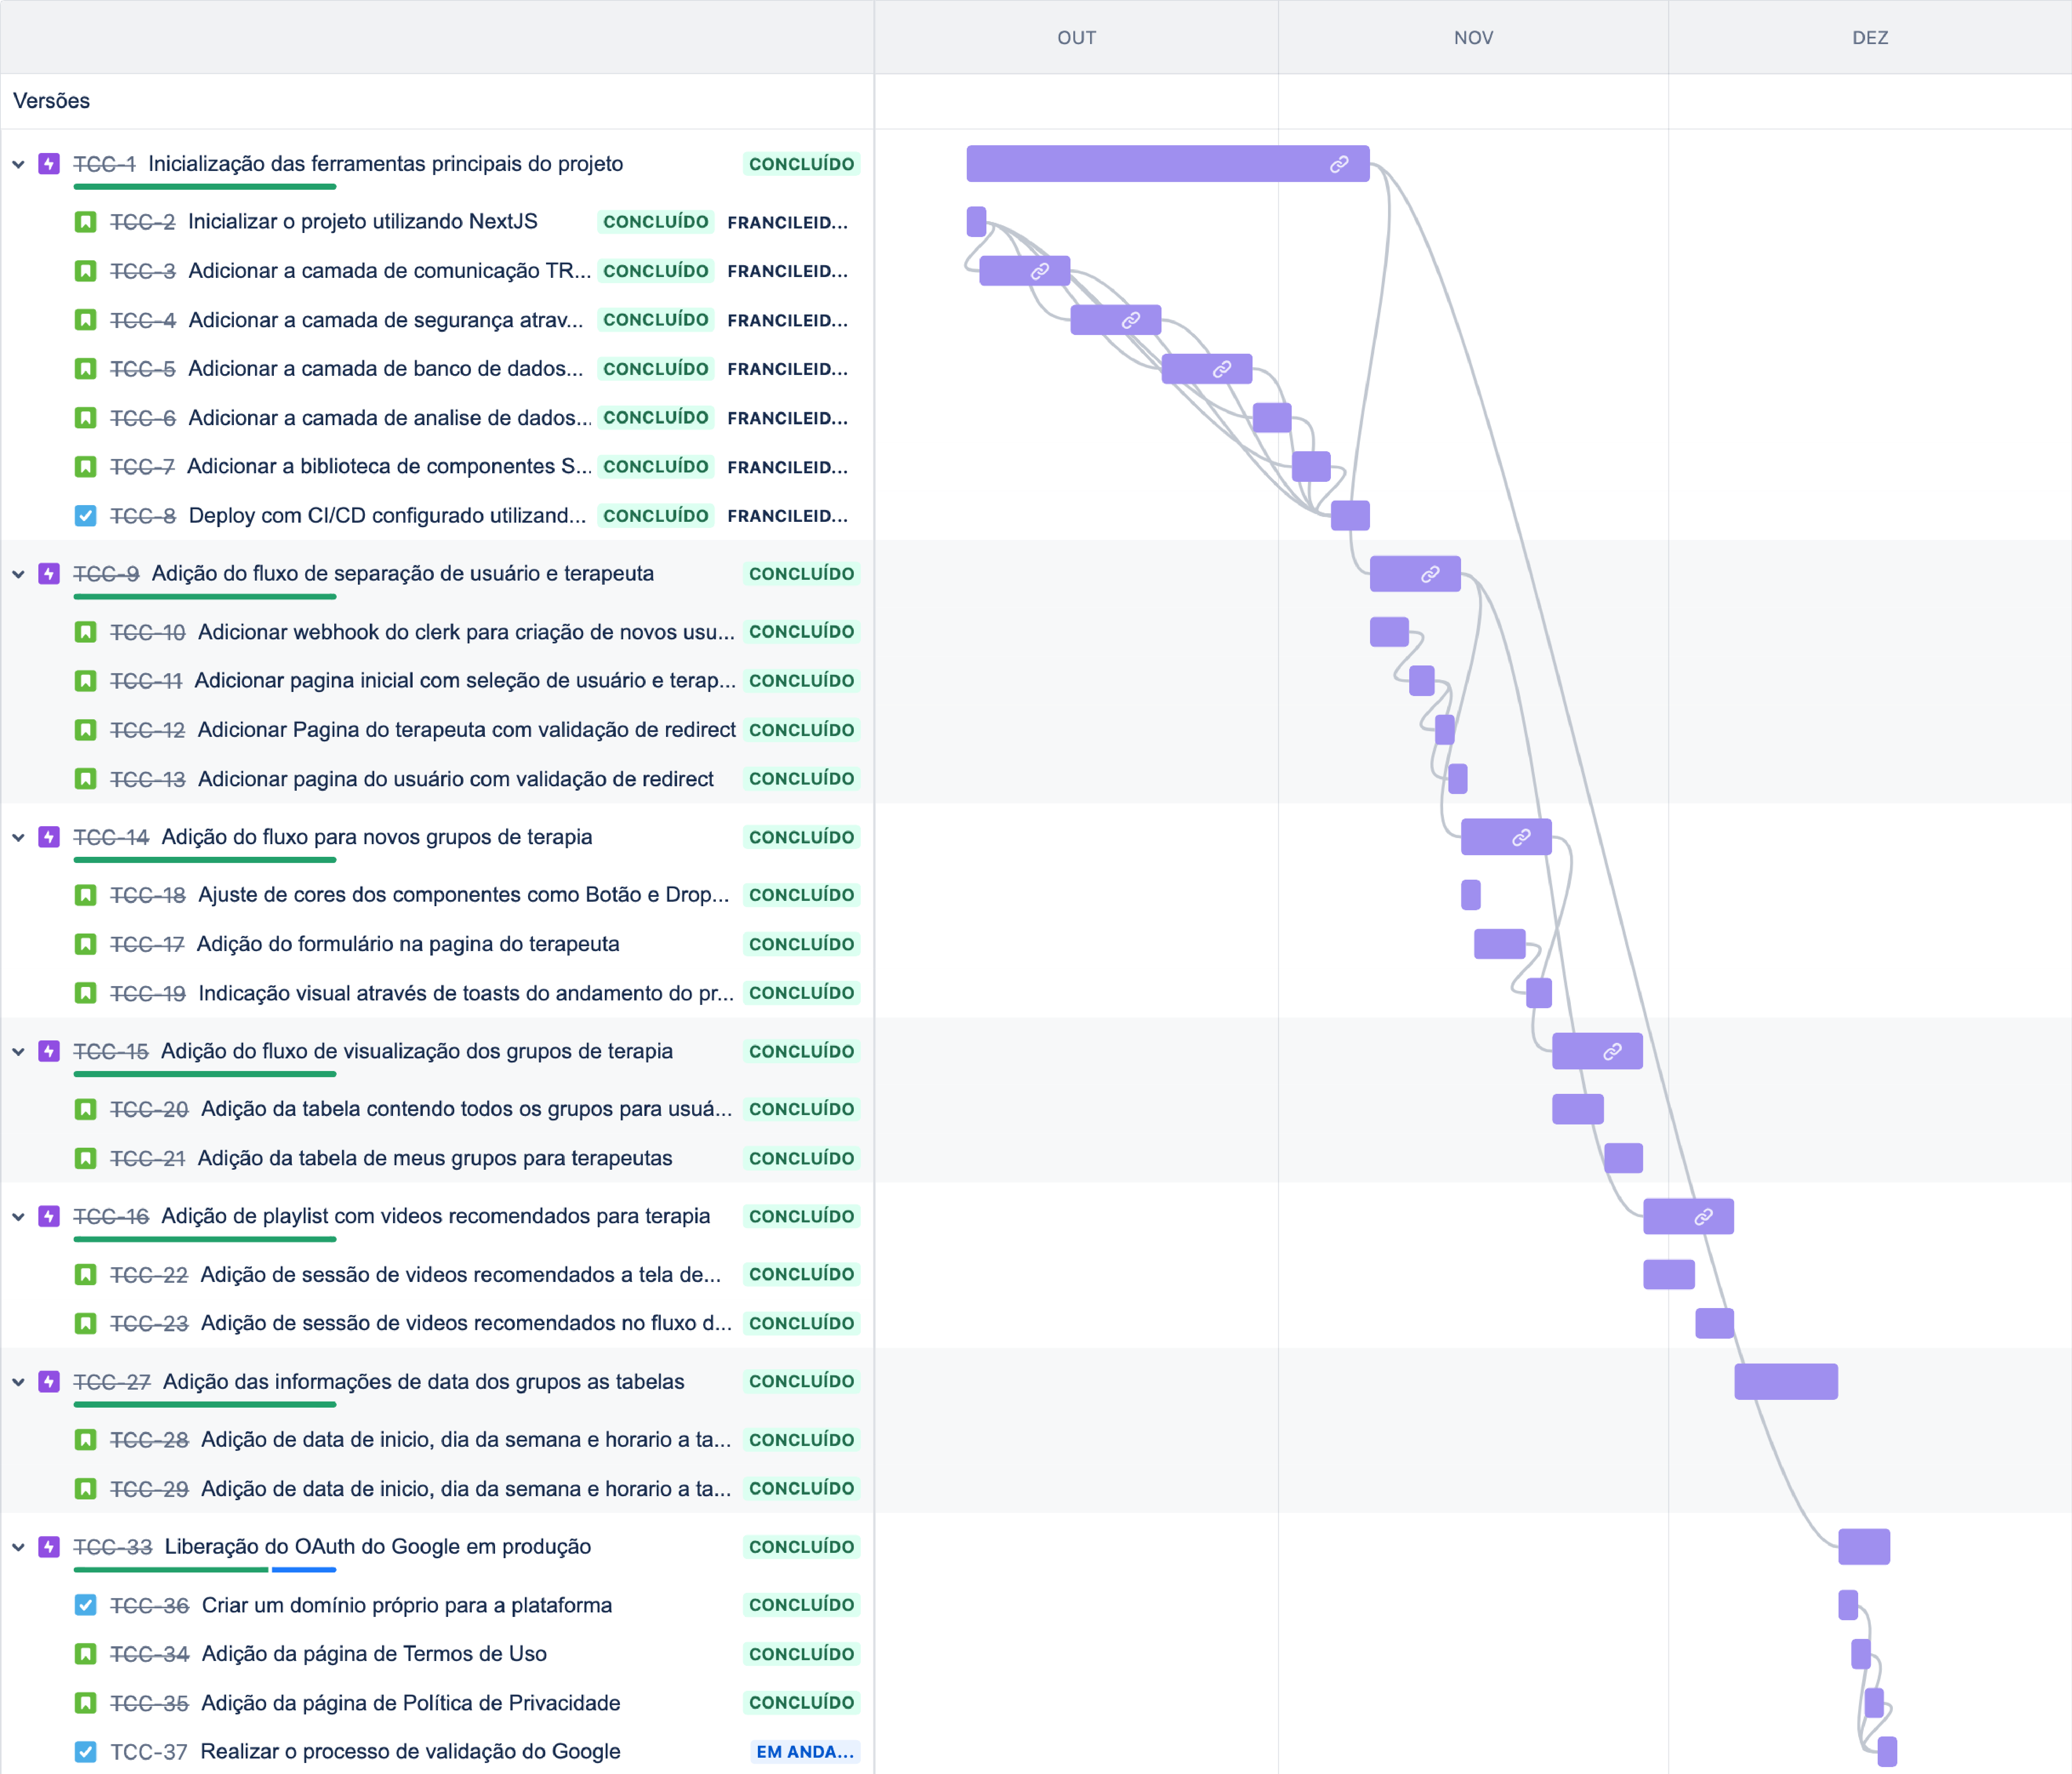
\includegraphics[scale=0.16]{latex/figuras/fluxojira.pdf}
    \label{fluxojira}
    \caption[Fluxo de Desenvolvimento do Projeto]{Fluxo da Linha do Tempo no Jira Software}
    \label{fig:enter-label}
\end{figure}\pagebreak

    A linha do tempo do Jira organiza essa evolução de forma sistemática.
    Cada \textit{story} concluída contribui para a evolução do projeto. Integrada à execução ágil, destaca marcos importantes. Uma narrativa dinâmica surge, revelando não apenas o caminho percorrido, mas também o potencial futuro da plataforma online.

    Essa abordagem prática e visual oferece uma compreensão clara do progresso e flexibilidade para ajustes ágeis, garantindo uma construção adaptável e alinhada às necessidades dos usuários da Terapia Comunitária Integrativa Online.

    




\subsection{Ferramentas Principais do Projeto}

\begin{enumerate}

    \item\textbf{Inicialização do projeto utilizando Next.js}
    
    Para dar início ao projeto, foi optado pelo gerenciador de pacotes PNPM e pelo \textit{framework} Next.js. A inicialização do projeto foi realizada através do comando:

\begin{verbatim}
    pnpm create next-app@latest
\end{verbatim}
    
    Na sequência, foram feitas seleções específicas, conforme ilustrado abaixo:
    
\begin{figure}[!ht]
    \centering
    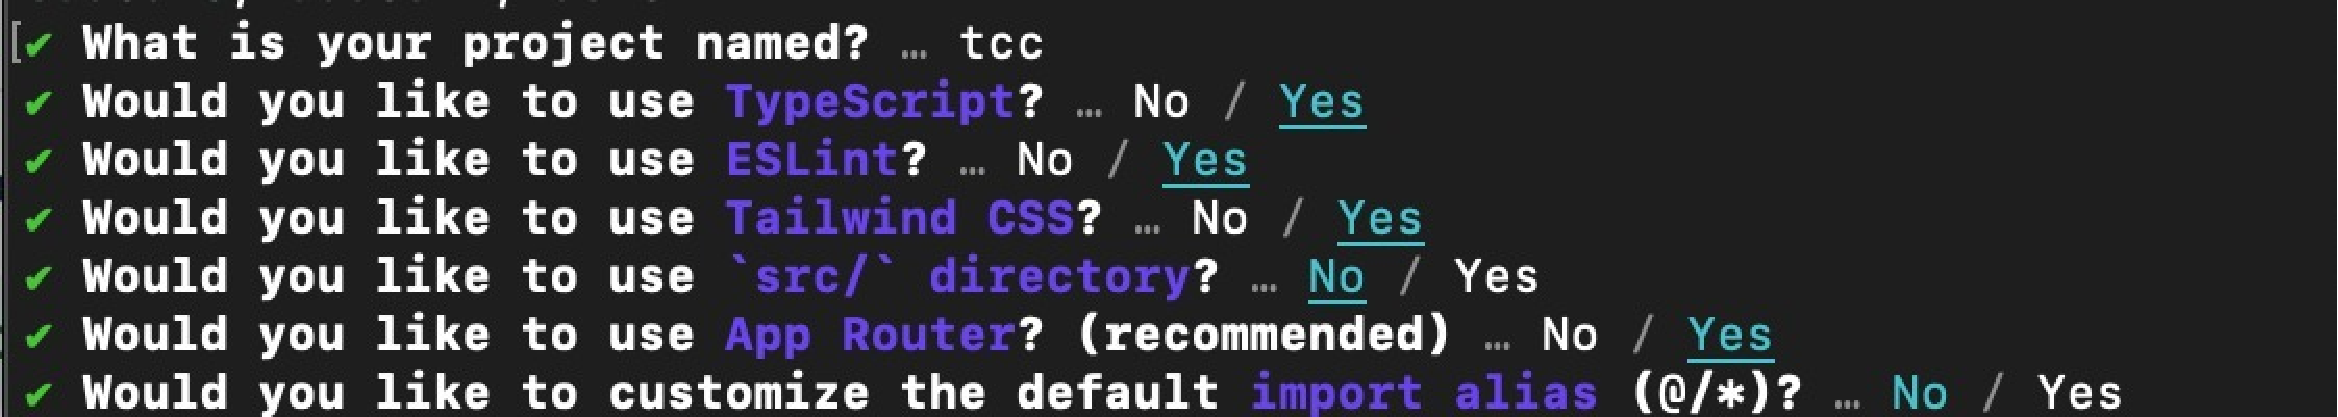
\includegraphics[scale=0.38]{latex/figuras/nextjs.pdf}
    \caption[Ferramentas Principais do Projeto]{Sequência de comandos de configuração Next.js}
    \label{fig:enter-label}
\end{figure}

    \item\textbf{Implementação da Camada de Comunicação TRPC entre Front-end e Back-end}
    
    A inclusão da camada exigiu a adição de pacotes por meio do comando:
    
\begin{small}
\begin{verbatim}
pnpm add @trpc/client @trpc/react-query @tanstack/react-query @trpc/server
\end{verbatim}
\end{small}

    Posteriormente, uma pasta denominada \textbf{Server} foi criada na raiz do projeto. Essa pasta contém a lista de rotas, suas respectivas lógicas e a estrutura básica do TRPC.\\Dentro da pasta \textbf{App}, foi criada uma subpasta chamada \textbf{api}. No contexto do Next.js, essa pasta atua como \textit{endpoints} externos capazes de receber chamadas HTTP, expondo todas as rotas TRPC.\\ 
    Para conectar o front-end às rotas TRPC e permitir o acesso às chamadas, foi necessário criar uma pasta chamada \verb|_trpc|, na estrutura do Next.js. Usando o \textit{App router}, as pastas com \verb|_| \textit{(underline)} na frente não são acessíveis externamente. Dentro desta pasta, foi estabelecido um provedor de TRPC que envolve a aplicação por completo, por meio do \textit{layout} da raiz e um arquivo de \textit{serverClient} que habilita componentes \textit{server side rendered} (SSR) a também utilizarem as rotas TRPC.
    
    \item\textbf{Camada de Segurança com a Utilização da Ferramenta Clerk}
    
    Para fortalecer a segurança, foi optado por integrar a ferramenta Clerk, conhecida por sua robusta estrutura de autenticação. A inclusão do Clerk foi realizada através do seguinte comando:
    
        \begin{verbatim}
                    pnpm add @clerk/next.js
        \end{verbatim}
    Posteriormente, as seguintes etapas foram efetuadas:
        \begin{enumerate}
            \item Ajuste do arquivo trpc dentro da pasta \textit{server} para criar um novo tipo de procedimento protegido por autenticação.
            \item Introdução de um \textit{middleware} na pasta raiz para determinar quais rotas devem ser públicas ou protegidas.
            \item Adição de uma nova rota à pasta \textbf{api}
            para receber \textit{webhooks} do sistema.
            \item Implementação da página de criação de conta e de login.
            \item Incorporação de um provedor ao \textit{layout} da raiz, garantindo que toda aplicação passe pelo processo de validação de rotas. Em casos de rotas protegidas, usuários não autenticados são redirecionados.
        \end{enumerate}
    
    \item\textbf{Camada de Banco de Dados com o Uso do ORM Prisma e MySQL Hospedado no \textit{PlanetScale}}\\
    
    Na camada de banco de dados, foi escolhido o \textit{PlanetScale}, um banco de dados MySQL em nuvem com um plano gratuito adequado para projetos pequenos. Para estabelecer a conexão entre o serviço e o banco de dados, o Prisma foi selecionado como ORM, devido à sua praticidade e ferramentas como o Prisma Studio e Prisma Migrate, facilitando o acesso ao banco e a migração de tabelas, respectivamente.\\\\
    A escolha do Prisma também levou em consideração a flexibilidade para futuras mudanças na escolha do banco, como a possibilidade de migrar para o \textit{PostgreSQL}. Nesse cenário, bastaria alterar o esquema no Prisma. Para incorporar o Prisma ao sistema, o seguinte comando foi executado:

    \begin{verbatim}
                    pnpm dlx prisma init
    \end{verbatim}
    
    Em seguida, foi ajustado o esquema, gerado automaticamente, para garantir compatibilidade com o \textit{PlanetScale}. Adicionalmente, o banco de dados foi inserido no contexto do TRPC, possibilitando seu uso em qualquer procedimento TRPC.

    \item\textbf{Camada de Análise de Dados de Uso com a Plataforma \textit{PostHog}}\\
    
    Para realizar a análise de uso, foi escolhido a ferramenta \textit{PostHog Cloud}, conhecida por registrar sessões do usuário, analisar eventos e monitorar fluxos de uso. A integração da biblioteca foi feita por meio do seguinte comando:
    
    \begin{verbatim}
                    pnpm add posthog-js posthog-node
    \end{verbatim}

    Em seguida, criada a pasta \textbf{\_posthog} dentro da pasta \textbf{App}. Nela, foi inserido um provedor, o qual foi adicionado ao \textit{layout} da raiz, possibilitando que todo o sistema gere eventos.
    
    \item\textbf{Biblioteca de componentes ShadCN UI}\\
    
    A opção pela biblioteca de componentes ShadCN UI foi motivada por sua coleção de componentes reutilizáveis com configuração de estilo. Para incorporar a biblioteca, foi necessário executar o seguinte comando:
    
    \begin{verbatim}
                    pnpm dlx shadcn-ui@latest init
    \end{verbatim}    
            
    Além disso, realizadas as configurações necessárias, conforme apresentado a seguir:
    
    \begin{figure}[!ht]
        \centering
        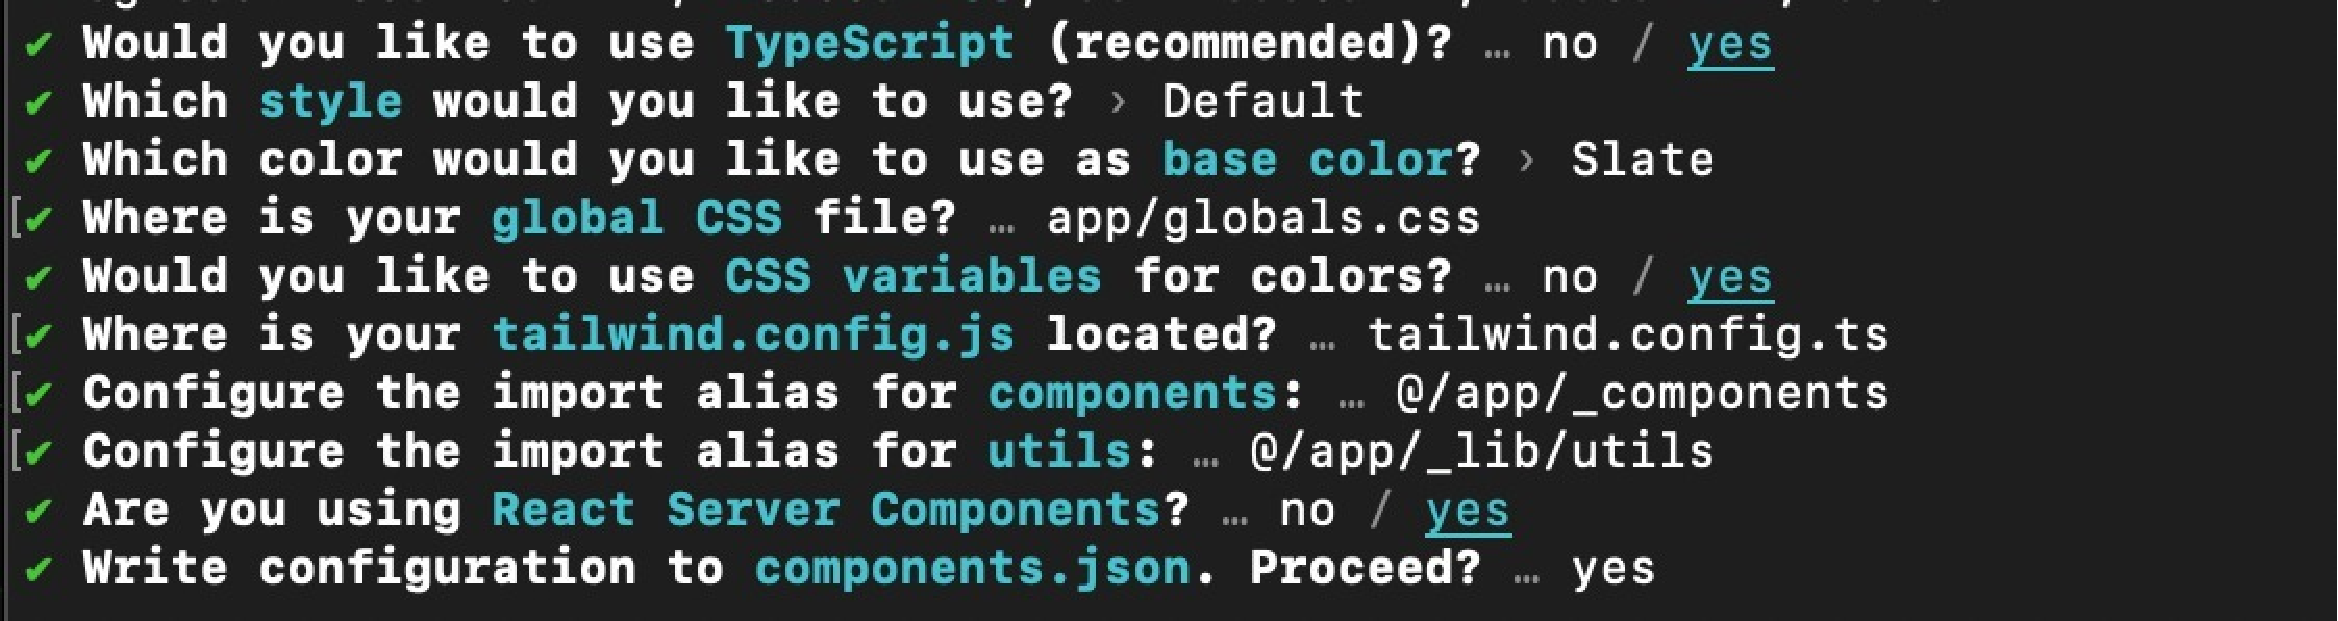
\includegraphics[scale=0.38]{latex/figuras/shadcnui.pdf}
        \caption[Ferramentas Principais do Projeto]{Sequência de comandos de configuração ShadCN UI}
        \label{fig:enter-label}
    \end{figure}

    Nesse processo, pode-se notar o uso das pastas \verb|_lib| e \verb|_components| para manter essas pastas como privadas.

    \item\textbf{Deploy com CI/CD configurado utilizando \textit{GitHub Actions} e Vercel}\\
    
    Com o projeto devidamente estruturado e as principais ferramentas configuradas, chegou o momento de realizar o primeiro \textit{deploy} na nuvem para iniciar as iterações. A escolha recaiu sobre a plataforma Vercel para hospedagem. O processo de \textit{deploy}, com o código no GitHub, foi simplificado, bastando conectar o projeto do GitHub à conta Vercel e inserir as variáveis de ambiente.
    
\end{enumerate}


\subsection{Fluxo de separação de usuário e terapeuta}
\subsection{Fluxo para novos grupos de terapia}
\subsection{Fluxo de visualização dos grupos de terapia}
\subsection{Playlist com videos recomendados para terapia}
\subsection{Informações de data dos grupos as tabelas}
\subsection{Liberação do OAuth do Google em produção}